\newpage
\section{背景及相关工作}
\setcounter{table}{0}
\setcounter{figure}{0}
\subsection{基于GPU的机器学习应用与CUDA}

\subsubsection{基于GPU的机器学习应用}
\par 随着当今机器学习,尤其是深度学习应用中数据量、网络结构复杂度的增长,该类应用对于硬件计算能力的要求也迅速增长。而在这类应用中,有许多密集的计算互相之间是没有数据/控制依赖的,也就是可以并行执行的;比如神经网络前向、反向传播中的权重矩阵计算,这些权重在同一轮计算中不存在耦合性;随机森林(Random Forest)中不同分类器的训练,这一特征可以利用到GPU处理中流这一特征;一系列聚类算法,包括DBSCAN、K-Means等;而图形处理单元(GPU)的设计初衷正是大规模并行计算,也因为GPU的计算能力,深度学习自上世纪末至今迅猛发展,同时GPU的运算性能以及相应的软件的发展也非常迅速。目前,GPU更多代表了通用处理单元(General Purpose)。
\par 当然,GPU上的编程模型与CPU上的模型有较大差别,为了方便程序员搭建模型,目前市面上的许多框架包括TensorFlow, PyTorch, PyChain等都更新了对GPU的支持。然而,这些框架方便了程序员的程序编写,抽象了底层硬件的细节,比如在CUDA中,线程块、线程束的调度以及相应寄存器文件的分配会对程序性能造成极大影响,然而这些特征都被框架抽象这就导致了硬件性能无法得到完全的发挥。且目前大部分框架都是基于老架构与老SDK编译,没有对新架构与新SDK做出优化。本文的目的也是在于挖掘出新架构的硬件以及对应的新的SDK中的代码翻译、指令执行等部分的特征以及相较老架构和老SDK的变化;根据分析得出的结论修改已有GPU程序的源码,尝试修改某些框架的源码,并给出实际的修改、编程时的建议。
\subsubsection{CUDA}
\par CUDA (Compute Unified Device Architecture)是由英伟达(Nvidia)针对图形处理单元开发的并行计算平台及对应的编程模型。在编写CUDA程序时,程序员通过在一些较为热门的语言包括C/C++、Python、MATLAB、Fortran中以关键字的形式加入扩展来描述并行行为\parencite{CUDAZONE}。下面将介绍CUDA程序的编程模型、编译过程与调用/执行方式。
\paragraph{编程模型}
\par 在介绍编程模型前,需要简要介绍一下Nvidia GPU的硬件结构。自顶向下的结构为:一块GPU芯片有若干图形处理簇(Graphics Processing Cluster, GPC),由外围总线进行调度管理;一个图形处理簇上有若干纹理处理簇(Texture Processing Cluster, TPC),需要注意的是以上两种结构在编写程序时并不暴露。一个纹理处理簇上有若干流多处理器单元(Stream Multiprocessor,SM)(在图灵架构中一个TPC仍只包含一个SM单元),这些流多处理器单元被一个线程块调度器管理,所有流多处理器单元通过全局内存总线和常量内存总线经过L2缓存共享全局内存与常量内存,这部分内存自费米架构以来有GDDR4、GDDR5、GDDR5X、GDDR6X、HBM、HBM2等类型。每个流多处理器单元中有若干个流处理器(Stream Processor,SP),因CUDA程序为SIMT(单指令多线程)并行方式,所以这些流处理器共享一个指令缓存,每个流处理器拥有自己的线程束调度器与寄存器文件;流处理器中包含若干种执行单元,有浮点单元,整数单元,在新架构中还加入了张量单元(Tensor Core),在RTX 2080TI上具体的参数为:一个SM包含64个单精度浮点算术单元,32个双精度浮点算术单元,64个32位整形算术单元,8个混合精度张量单元,4个线程束调度器和16个特殊功能单元;所有流处理器通过显存纵横矩阵(CrossBar)访问共享内存,或被称为L1缓存\parencite{EXPLORING},所有流多处理器共享L2缓存。
\par 因本文的工作主要基于C/C++完成,故只介绍CUDA C/C++的编程模型。在保证相关环境配置完成后,向C/C++源码中加入CUDA相关工具是十分方便的。首先需要确定哪些任务需要在CPU上执行,哪些在目标硬件GPU)上执行;选择的标准一般是考察其数据/控制依赖,依赖性小、计算密集的可以考虑在GPU上执行。确定完毕后编写CPU端和GPU端的函数,有如图\ref{Fig.1}中所示的三种函数。
\begin{figure}
	\centering
	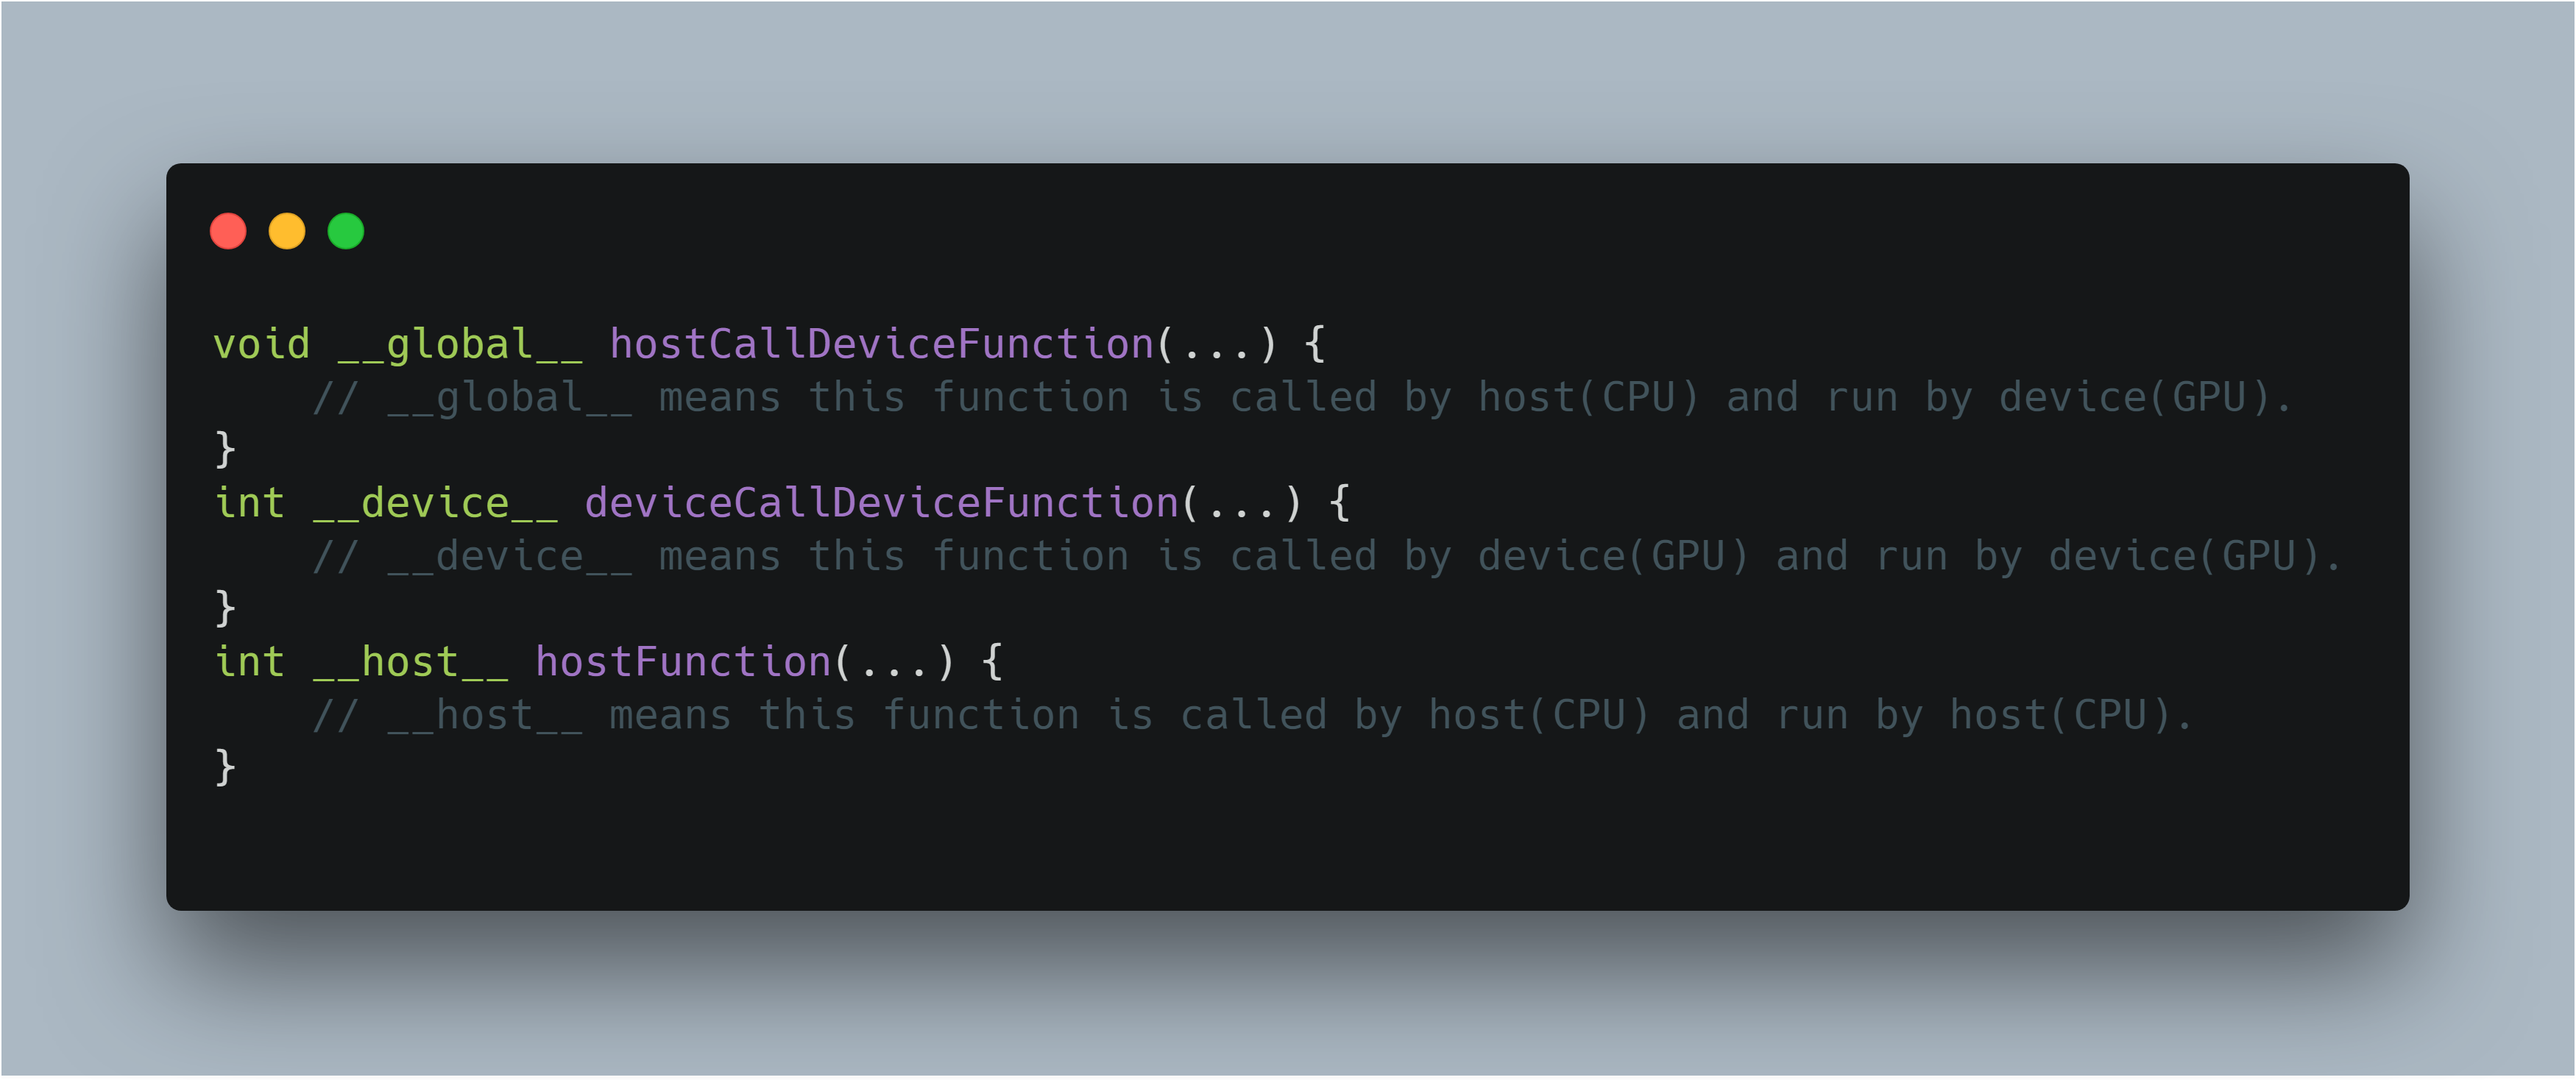
\includegraphics[width=15cm]{figures/CODE1.png}
	\renewcommand{\thefigure}{\arabic{section}-\arabic{figure} }
	\renewcommand{\figurename}{图}
	\caption{CUDA中的三种函数}
	\addtocounter{figure}{-1}
	\renewcommand{\thefigure}{\arabic{section}-\arabic{figure} }
	\renewcommand{\figurename}{Figure}
	\caption{3 types of function in CUDA}
	\label{Fig.2}
\end{figure}
\par 以上代码段加粗部分为CUDA关键字,对于函数有三种修饰:\_\_global\_\_, \_\_device\_\_, \_\_host\_\_. 分别代表被CPU调用运行于GPU、被GPU调用运行于GPU和被CPU调用运行于CPU的函数。其中被CPU调用运行于GPU的函数只能拥有void返回值,且所有运行于GPU的函数都不支持可变参数列表\parencite{EVENEASIER}。\_\_device\_\_和\_\_host\_\_关键字修饰的函数的调用方式与传统函数别无二致,\_\_global\_\_关键字修饰的函数调用方式如图\ref{Fig.4}所示。
\begin{figure}
	\centering
	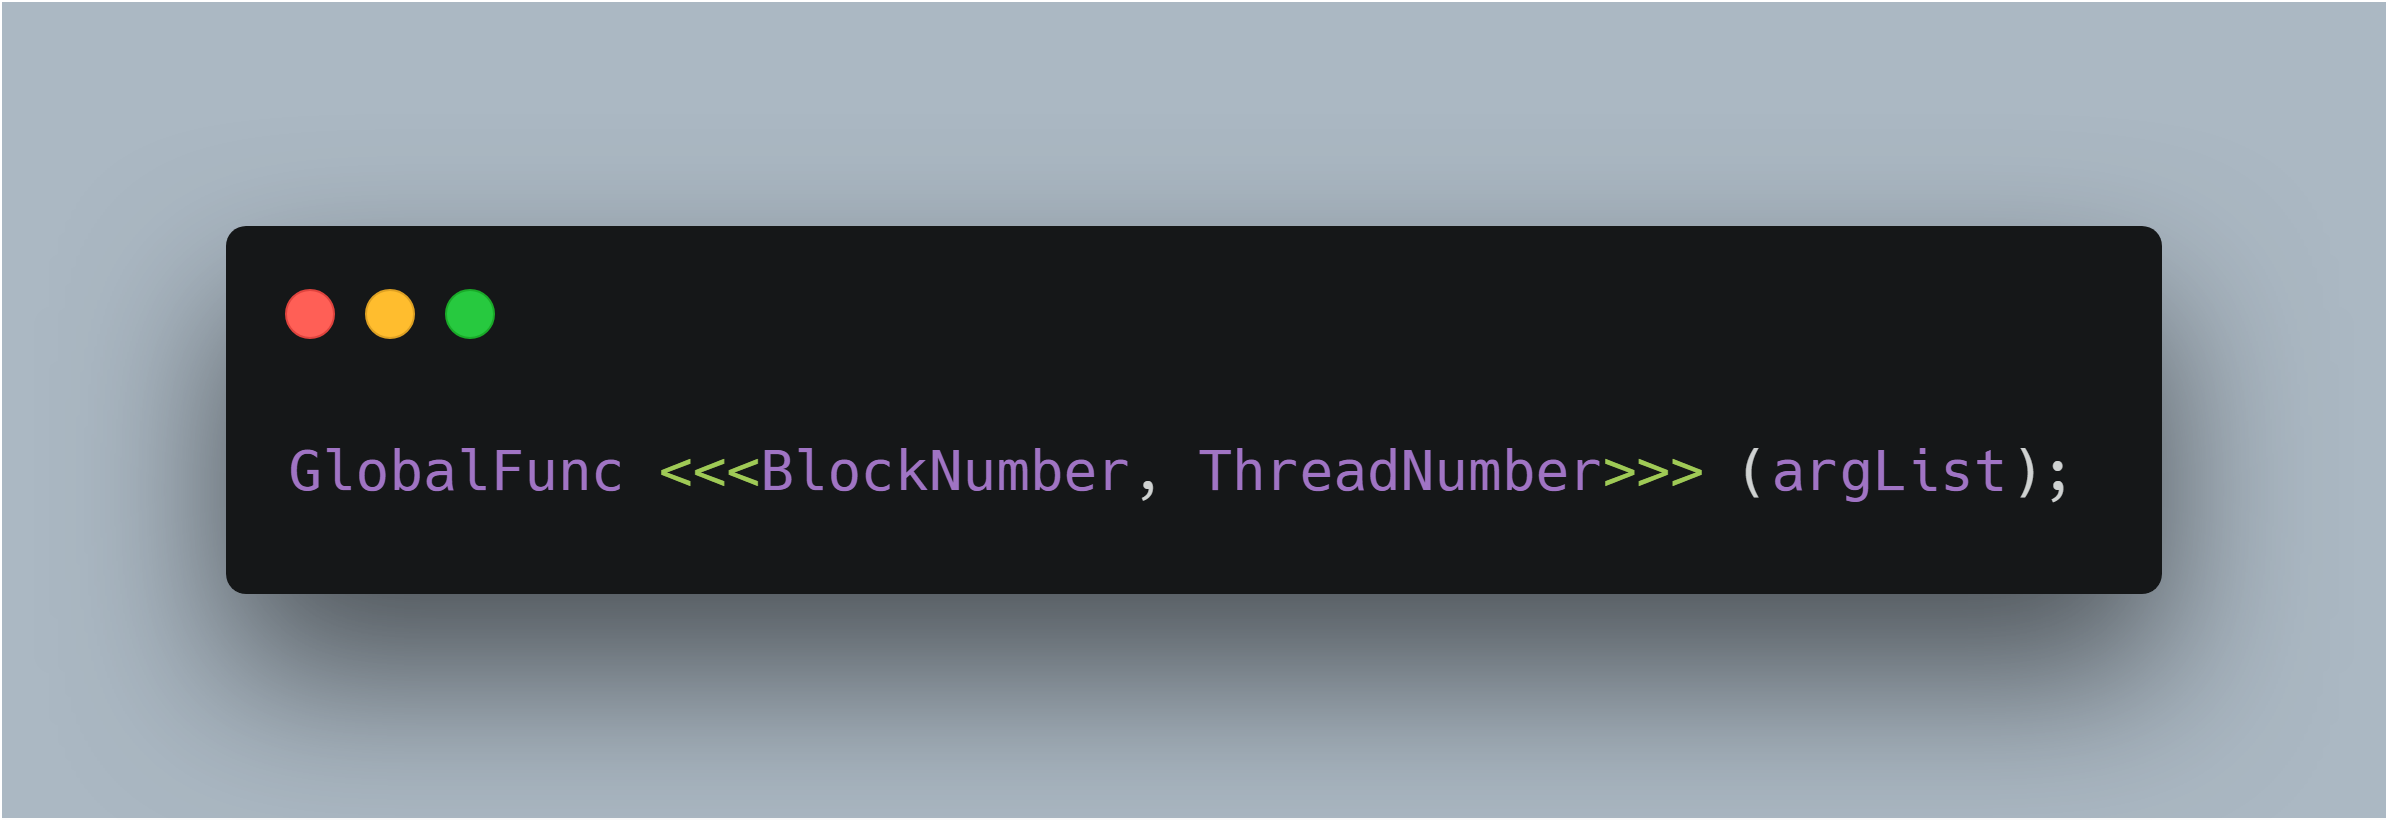
\includegraphics[width=15cm]{figures/CODE3.png}
	\renewcommand{\thefigure}{\arabic{section}-\arabic{figure} }
	\renewcommand{\figurename}{图}
	\caption{CUDA核函数调用方式}
	\addtocounter{figure}{-1}
	\renewcommand{\thefigure}{\arabic{section}-\arabic{figure} }
	\renewcommand{\figurename}{Figure}
	\caption{Invoking method of kernel function in CUDA}
	\label{Fig.4}
\end{figure}
BlockNumber和ThreadNumber分别代表要启动的线程块数目和每个线程块中线程的数目,这一部分取值对程序性能影响较大,之后会详细说明。

\par 之前提到了GPU端的缓存,CUDA程序的另一个重点是存储系统的管理。传统CPU编程模型中,寄存器、缓存等资源都是由CPU自行管理,而不开放给程序员。其原因在于CPU拥有的寄存器、缓存资源较为紧缺,为提高指令级并行能力,需要采用多队列乱序发射与寄存器重命名等技术。相对得,GPU有较为充足的物理寄存器、缓存资源,程序员也对这部分资源掌握有一定的控制权\parencite{CUDAPROG}。CUDA中的存储设备如表\ref{table-存储}所示。
\begin{table}
	\centering
	\renewcommand{\thetable}{\arabic{section}-\arabic{table} }
	\renewcommand{\tablename}{表}
	\caption{CUDA存储系统层级}
	\addtocounter{table}{-1}
	\renewcommand{\thetable}{\arabic{section}-\arabic{table} }
	\renewcommand{\tablename}{Table}
	\caption{CUDA storage system hierarchy}
	\begin{tabular}{cccc}
		\toprule
		项目				&	大小			&	延迟(时钟周期)	&	访问权限	\\
		\midrule
		寄存器文件		&	8KB-64KB/SM		&	$ 10^0 $	& GPU端	\\
		共享内存(L1,L2)	&	16KB-128KB/SM	&	$ 10^1 $	&	GPU端\\
		常量内存		&	N/A				&	N/A		&	N/A	\\
		纹理内存		&	N/A				&	N/A		&	N/A \\
		全局内存		&	-GB				&	$ 10^2 $	&	CPU端/GPU端 \\
		\bottomrule
	\end{tabular} \label{table-存储}
\end{table}
\par 需要注意的是,常量内存与纹理内存都是全局内存的一种虚拟地址形式。和常量内存一样,纹理内存也是一种只读内存;但是在缓存加载的行为方面,常量内存与传统方式一样,加载所访问数据单元的所在行的一部分单元,而纹理内存则加载所访问数据周围一个范围内的单元\parencite{THEDESIGN}。这样做的原因是在GPU进行图形运算时,处理某一像素点需要用到周围一个范围内所有像素点的信息比如进行抗锯齿作业时,而非只有一行,如图\ref{Fig.1}所示。采用这种结构能改善某些访问模式情况下程序的性能。
\par 这些内存的使用方式如图\ref{Fig.3}所示。寄存器和共享内存的使用方式很好理解,关于常量内存和纹理内存,由于他们是全局内存中的虚拟地址,故声明常量内存的语句也就是用了全局内存;纹理内存的使用则需要借助相应API。而一般的全局内存的读写权限同时开放给CPU和GPU,故需要使用特定的API进行访问。
\begin{figure}
	\centering
	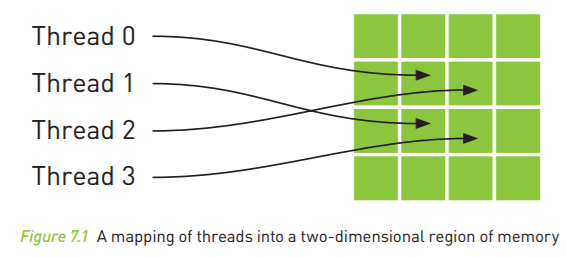
\includegraphics[width=15cm]{figures/Fig1.jpg}
	\renewcommand{\thefigure}{\arabic{section}-\arabic{figure} }
	\renewcommand{\figurename}{图}
	\caption{纹理内存}
	\addtocounter{figure}{-1}
	\renewcommand{\thefigure}{\arabic{section}-\arabic{figure} }
	\renewcommand{\figurename}{Figure}
	\caption{Texture Memory}
	\label{Fig.1}
\end{figure}
\begin{figure}
	\centering
	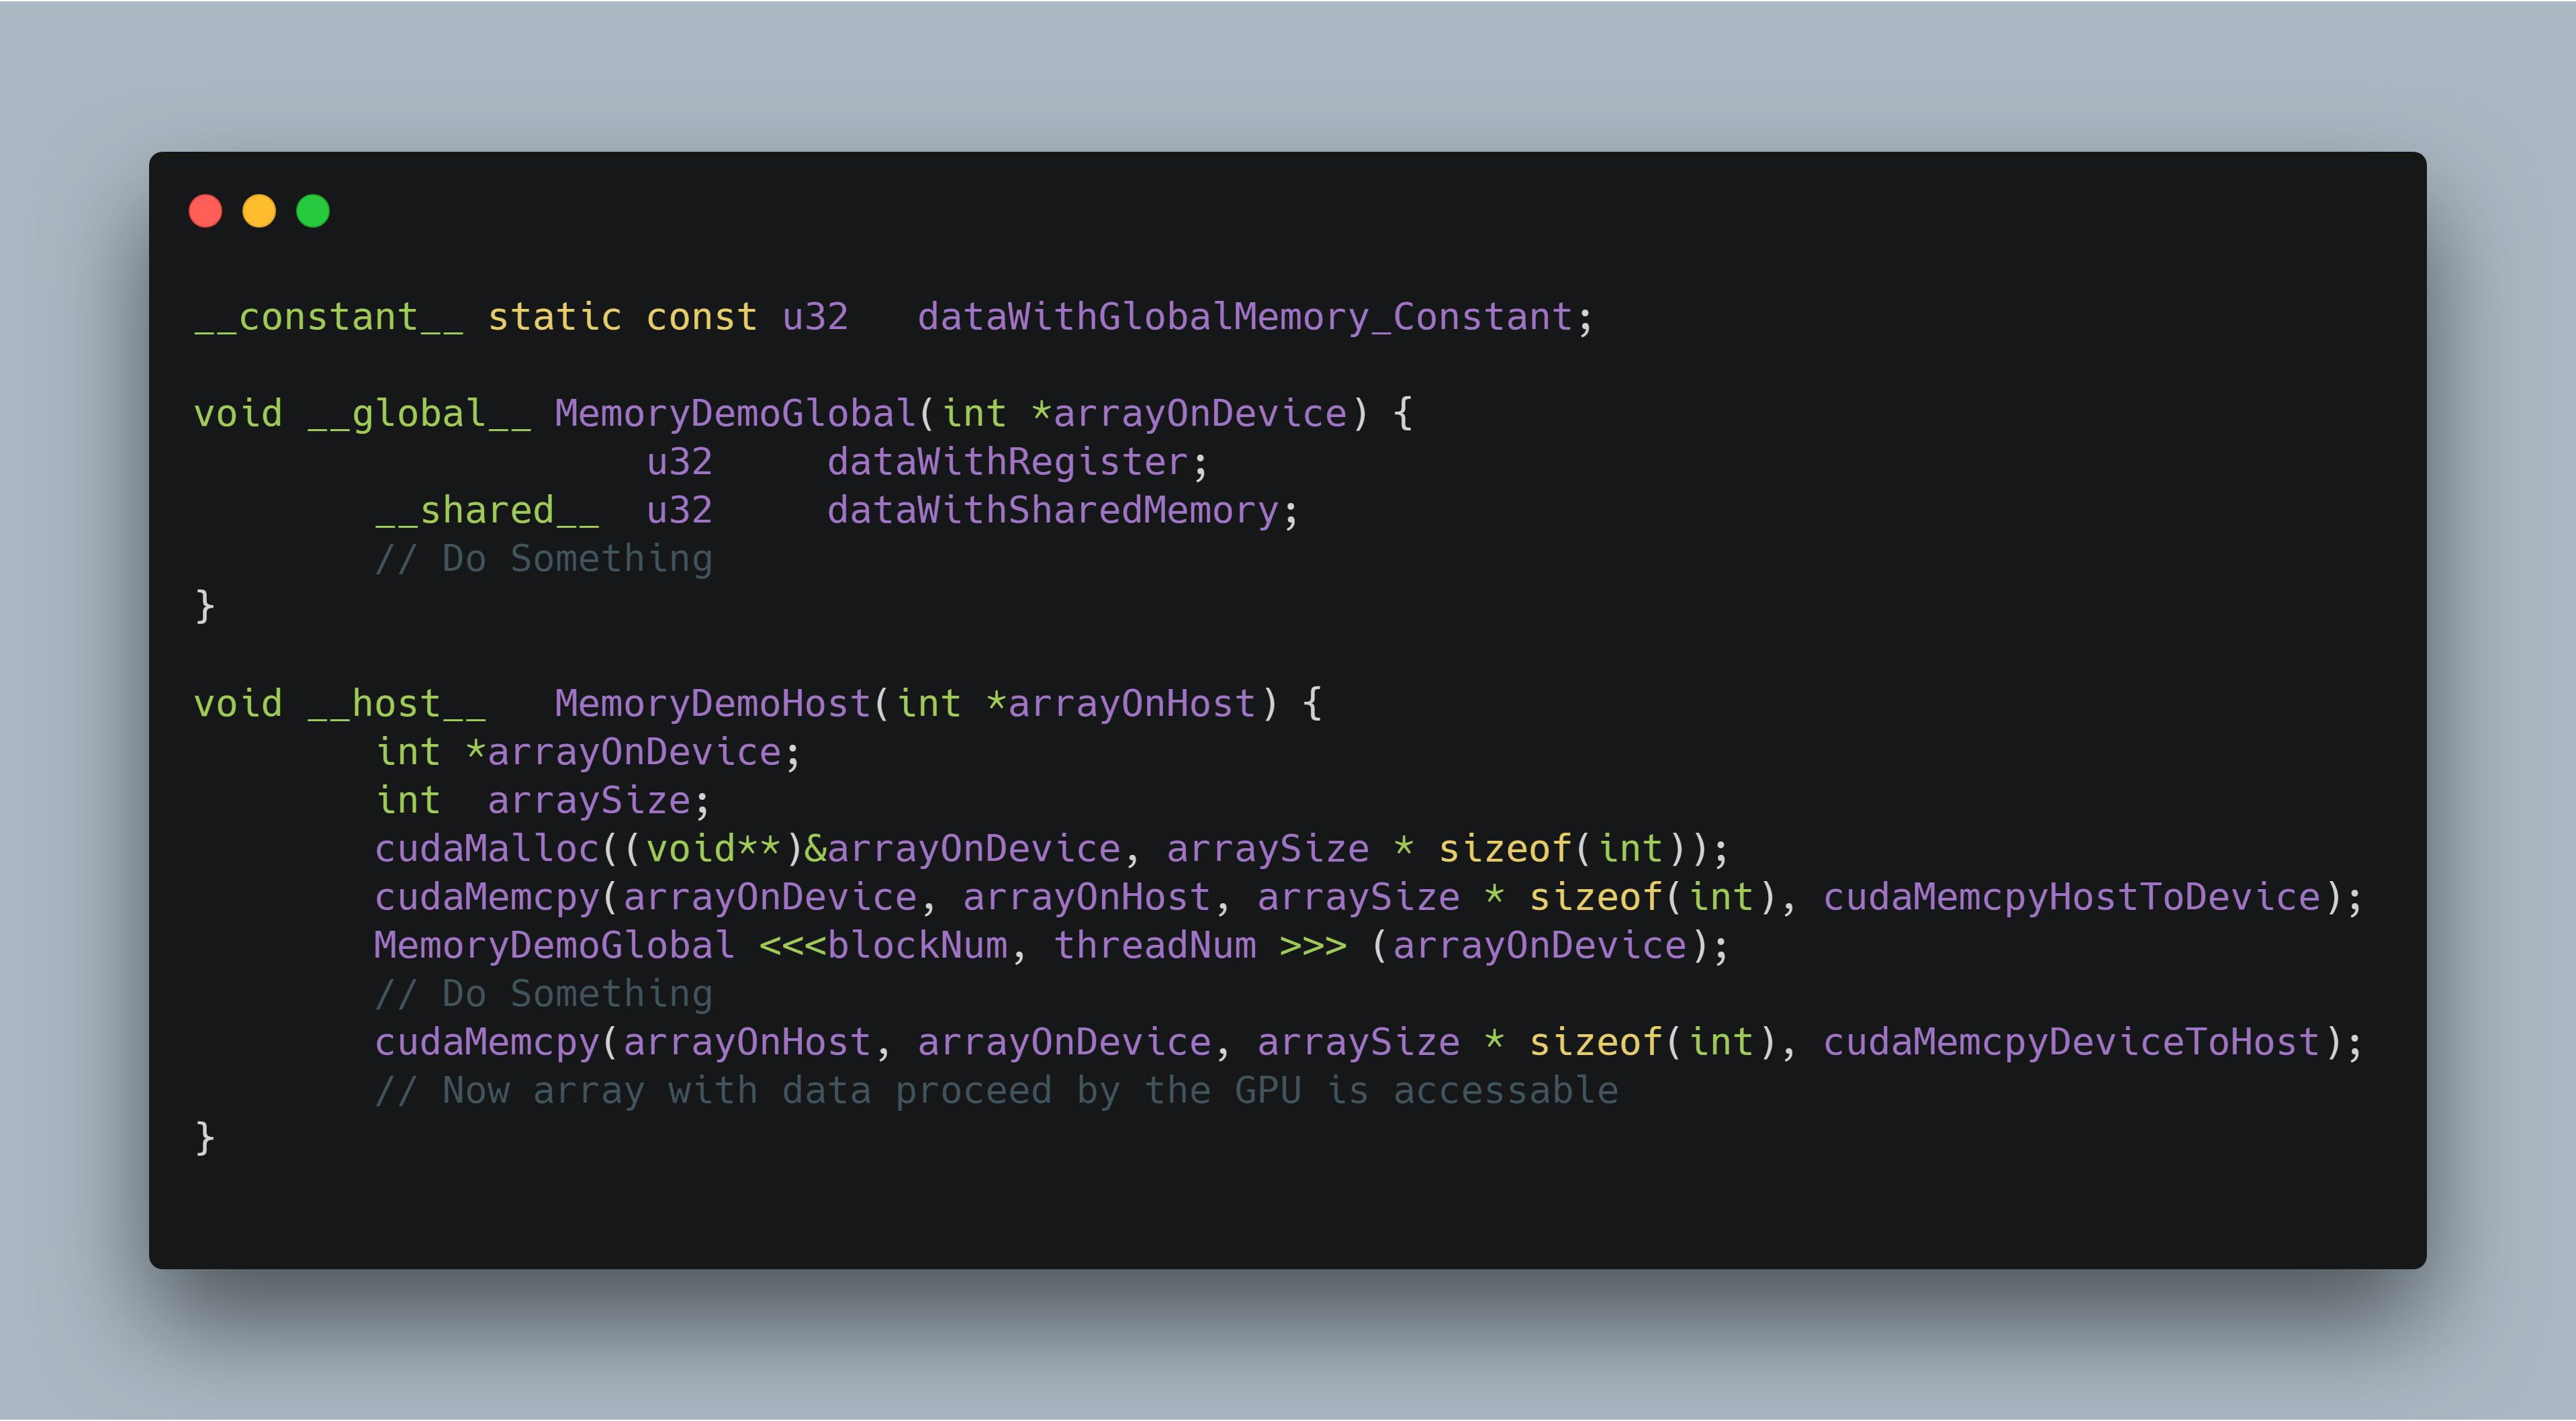
\includegraphics[width=15cm]{figures/CODE2.png}
	\renewcommand{\thefigure}{\arabic{section}-\arabic{figure} }
	\renewcommand{\figurename}{图}
	\caption{不同存储单元的使用方式}
	\addtocounter{figure}{-1}
	\renewcommand{\thefigure}{\arabic{section}-\arabic{figure} }
	\renewcommand{\figurename}{Figure}
	\caption{Methods of using different storage unit}
	\label{Fig.3}
\end{figure}
\paragraph{编译方式}
\par CUDA程序的编译较为简单,只需使用$ nvcc $对源文件进行编译生成可执行文件。首先将从C/C++/CUDA文件编译生成PTX中间代码,再从PTX中间代码生成SASS机器代码。本实验中由于需要观察、研究具体GPU代码的生成方式、特征,故在编译时加入$ --keep $保留编译产生的PTX中间代码文件。而SASS机器代码则在NVIDIA的支持下通过捕捉CUDA应用的指令流获得。
\paragraph{运行模式}
\par 关于如何从CPU端(host)启动GPU端(device)的函数将在下一节通过CPU端应用程序的反汇编代码详细描述,这一节仅介绍GPU相关的部分。
\par 根据弗林分类法\parencite{FLYNN},计算机系统可以分为SIMD, MIMD, SISD, MISD等类型,目前多核心CPU系统就是MIMD系统。而NVIDIA的GPU系统被称为SIMT(单指令多线程),与SIMD(单指令多数据)有所不同。在这种模型中,一条指令并非仅仅代表一个固定的功能,而是代表执行这一指令的类型、使用的管道/流水线。线程需要执行的具体操作需要编写相关内核代码。直观的特征便是再PTX中间代码和SASS机器代码中,所有的逻辑操作指令都是$ lop/lop3 $,通过后缀$ .and/.or, .sync/.async $指明具体运算和调度特征。所以,在SIMT模型中,内核程序读入统一的数据,程序代码根据需要进行不同操作;实际调度时不同操作通过重复指令流按顺序发射,只不过运算单元会屏蔽无关线程。
\par 首先需要介绍一下计算能力,此处计算能力指的是GPU中流多处理器(SM)支持的运算的等级,分为Major和Minor等级,可以等价为流多处理器的代号,所支持的运算不同。其中Major代号代表架构的更新,这也会带来许多新的硬件支持的运算,而Minor代号则代表同一架构下不同定位的流多处理器产品。如伏特架构的计算能力为7.2,图灵架构的计算能力为7.5,Major代号一样就代表这两种架构其实并无太大修改,而Minor代号则代表伏特架构中流多处理器的类型是Heavy,图灵架构中流多处理器的类型是Lite。Lite和Heavy一般用于区分消费级/工作站级GPU,分别对应GeForce和Tesla代号。
\par 基于GPU的应用与传统的基于CPU的应用在运行方式上有较大差别,主要有以下几点。
\begin{itemize}
	\item GPU中由大量的物理寄存器,达几十~几百KB,且都能在1个时钟周期内访问,而CPU中物理寄存器资源极为有限。故在进行上下文切换时,GPU只需更改寄存器文件指针来切换,而CPU需要使用堆栈保存上下文。
	\item CPU仅仅支持数十个硬件线程,而GPU则支持数千个硬件线程。在GPU上开启过少的硬件线程会极大降低硬件使用率,进而导致性能降低。具体开启线程数量取决于硬件SM最大并发线程数、最大并发线程束数和最大并发块数等。表\ref{table-占用率}显示了在不同计算能力上开启不同数量的线程时设备的利用率以及所能开启包含该数量线程的线程块的数量。\\
	\begin{table}
	\centering
	\renewcommand{\thetable}{\arabic{section}-\arabic{table} }
	\renewcommand{\tablename}{表}
	\caption{可分配线程数与占用率的关系}
	\addtocounter{table}{-1}
	\renewcommand{\thetable}{\arabic{section}-\arabic{table} }
	\renewcommand{\tablename}{Table}
	\caption{Available thread number and corresponding occupancy rate}
	\begin{tabular}{cccccc}
		\toprule
			&	1.0	&1.2	&2.0	&2.1	&3.0 \\
		\midrule
		64	&	67\%, 8		&	50\%, 8		&	33\%, 8		&	33\%, 8		&	50\%, 16	\\
		96	&	100\%, 8	&	75\%, 8		&	50\%, 8		&	50\%, 8		&	75\%, 12	\\
		128	&	100\%, 6	&	100\%, 8	&	67\%, 8		&	67\%, 8		&	100\%, 10	\\
		256	&	100\%, 3	&	100\%, 4	&	100\%, 6	&	100\%, 6	&	100\%, 8	\\
		512	&	67\%, 1		&	100\%, 2	&	100\%, 2	&	100\%, 3	&	100\%, 4	\\
		1024&	N/A, N/A	&	N/A, 1		&	67\%, 1		&	67\%, 1		&	100\%, 2	\\
		
		\bottomrule
	\end{tabular} \label{table-占用率}
	\end{table}
	可见,随着计算能力的增长,一个流多处理器上所能容纳的线程束月俩月多。在充分利用寄存器文件和共享内存(L1缓存)的情况下开启线程数越多,设备利用率越高。然而过多的线程会导致资源紧缺,在实际使用中应当根据硬件参数,问题规模做出调整。
\end{itemize}
\par 在CUDA程序中,32个线程被组织成一个线程束(warp),作为基本的调度单元,具有各自的物理寄存器,也就是说线程束中32个线程一般情况下都会执行相同指令流,为SIMD模式。在目前的图灵架构中,线程束仍然是同步的单位,即线程束之间可以保证同步,线程束内部线程无法保证同步。在下一代安培架构(Ampere)则引入$ Arrive-Wait $模式以实现线程级别同步,以提高CUDA程序的灵活性。 
\par 若干个线程束被组织为一个线程块(block),在下一代安培架构中将添加一个线程束组的层级(warp group),由四个线程束组成,但该层级仅为大规模通用矩阵乘法运算所用(Ultra MMA),且本代架构还未应用,这里不做讨论。线程块中的线程束可以通过\_\_syncthread()进行同步,线程块中的线程能够访问共享内存进行数据交换。一个线程块被分配在一个流多处理器上执行,一个流多处理器能分配多个线程块。
\par 若干个线程块被组织成一个线程网格(grid),线程网格可被看作一个分配给GPU的任务。
\par 表\ref{table-粒度}详细说明了CUDA应用中不同不同粒度的线程组织形式。
\begin{table}
	\centering
	\renewcommand{\thetable}{\arabic{section}-\arabic{table} }
	\renewcommand{\tablename}{表}
	\caption{线程组织形式}
	\addtocounter{table}{-1}
	\renewcommand{\thetable}{\arabic{section}-\arabic{table} }
	\renewcommand{\tablename}{Table}
	\caption{Type of organizing threads}
	\begin{tabular}{ccc}
		\toprule
		粒度	&	调度者	& 	分配给 \\
		\midrule
		warp		&	流多处理器内部调度器	&	流处理器(Stream Processor)\\
		block(CTA)	&	TPC调度器(MPC)		  &		流多处理器(Stream Multi-processor)\\
		grid		&	GPC调度器(GPM)		  &		TPC(Texture Processing Cluster)$ * $\\
		kernel		&	CPU, PCIe			&		GPC(Graphics Processing Cluster)	\\	
		\bottomrule
	\end{tabular} \label{table-粒度}\\

$ * $ 在本世代图灵架构及以前,TPC与SM可以等价,因为一个TPC上仅包含一个SM,然而自下一代安培架构开始,一个TPC中将会有若干个SM。虽然本文研究的图灵架构的硬件在逻辑上SM与TPC等价,但在硬件上还是会做区分,故在表中详细写出\parencite{BLOCKDIAG}。
\end{table}
\par 以上内容介紹了CUDA中的线程组织形式,接下来将介绍调度方式。一个任务也可被看作一个线程网格,由CPU分配该GPU上的GPC,在线程块级别的调度上,GPU将遵循负载均衡的原则在某一线程块工作结束释放资源时调度下一线程块。在线程级别的调度上,一般情况下将以32个线程为单位进行调度,这32个线程执行同一指令流处理不同数据流;而在产生分支时,与CPU使用分支预测处理分支指令,遇到预测错误则清空流水线不同,GPU采用线程束分化(CBU指令)的方式处理;线程束分化机制下每一个分支都会有线程执行到,在分支结束处聚合。对于不满足分支条件的线程,GPU调度器将这些线程设置为未激活状态,继续向下执行。然而,硬件调度器每周期只能为一个线程束取到一条指令,这意味着线程束中部分线程会被阻塞,从而导致利用率下降,性能下降。在编写程序时,应尽量避免线程束内部线程分化,而在CUDA中存在非常细致的线程、线程块、线程网格ID,故根据这些ID控制分支使得线程束内部线程分化尽可能少时可行的\parencite{DIVER}。自麦克斯韦架构(Maxwell)以来,指令集中添加了CBU(Convergence Barrier Unit)指令以保持通过同一分支的线程被组织在一起,就是为了减少线程束分化带来的性能下降\parencite{THREADS}。
\par 最后将介绍CUDA中流这一机制以及相应的锁页内存。CUDA流可被看作一个GPU操作队列,该队列中的操作将会按顺序执行,这一特点使得在实际编写程序的过程中可以通过调整不同操作的顺序,如访存、密集的计算、写会等来隐藏数据依赖和控制依赖带来的延迟\parencite{STREAM},通过异步操作(ASYNC)提升任务级并行度。CUDA流需要在支持设备重叠的GPU上运行。设备重叠只GPU能够在执行一个核函数时在设备和主机间进行数据交互。
\par 而为了支持CUDA流,所有涉及流的内存需要字啊锁页内存上进行分配。锁页内存正如其字面含义,是分配在显存上、不允许被移动或被换页到磁盘上的设备内存。其好处是允许GPU上的DMA控制器绕过CPU直接请求主机传输数据,在延迟更低的基础上支持设备重叠。若不适用锁页内存,DMA控制器在定位内存页面时会造成困难。本文中,TensorRT中利用了CUDA流的特性,将在相应章节介绍。
\par 这一章从线程组织形式到调用运行方式介绍了CUDA应用,对实验中进行设备相关的优化有较大的帮助。
\subsection{目前展开的工作}
\par 本文的研究同时涉及硬件和软件:Nvidia新架构的GPU与使用GPU加速计算的机器学习应用,注意这里的机器学习应用并不只是现在大行其道的深度学习,还包括传统的基于概率模型的方法等。
\par 在近年来深度学习迅猛发展之前,关于使用GPU并行化机器学习算法的研究就已有很多,甚至可以说正是基于GPU的强大并行计算能力,深度学习才能发展如此迅速。早在2005年,D. Steinkraus等人便对在GPU上实现机器学习算法进行了研究, 当时实现的算法是OCR,如今OCR能够非常快速、方便地通过各种框架、语言实现。然而这一研究奠定了使用GPU加速机器学习应用的基础\parencite{GPUFORML}。之后的几年中,除去OCR外,基于GPU的各种并行机器学习算法包括kNN\parencite{KNNG},支持向量机\parencite{SMOSVM}都慢慢成熟。由于贝叶斯网络的精确推理是个NP难的问题,其性能受限于硬件水平,然而根据Md Vasimuddin等人的研究\parencite{BAYESINF},通过并行方法将延迟降低了许多。由于传统机器学习方法有着延迟低、模型小、训练时间短、可解释性强等优点,在深度学习迅猛发展的今天,传统机器学习方法仍然占有很大的市场,故评估GPU对传统机器学习加速的性能是十分有必要的。本文中在评估传统机器学习的部分便采用了并行的支持向量机算法(SMO-SVM),如今,不管是在工业生产领域还是学术研究领域,该算法仍占有一席之地。
\par 之后不久,深度学习、神经网络便迎来了爆炸式的发展。实际上在二十世纪末,便已经有完整的神经网络算法的理论基础;在1979年,日本学者福岛邦彦提出了Neocognition模型,其中使用多层网络以及神经元对图像特征进行提取和筛选被认为是启发了卷积神经网络的开创性研究\parencite{JAPANESSAY}。1989年,LeCun首次在论文中提出了“卷积”一次,卷积神经网络因此得名\parencite{LENET}。在1993年,贝尔实验室对LeCun的工作进行了代码实现,并大量部署于手写支票识别系统,然而限于当时计算能力低下,基于神经网络的研究也停滞在了理论阶段,其主要原因便是网络中需要训练的参数太多,网络结构复杂,在当时没有芯片能满足如此高的性能要求\parencite{NNML}。然而,随着高性能GPU芯片的出现,基于神经网络的方法正如日中天地发展。从TinyCNN等较轻量级、功能单一的库,到TensorFlow、PyTorch、Caffe、Chain等完整、易于使用的框架,这些工具或是本身就是基于GPU编写的,或是慢慢更新对GPU的支持;目前市面上的绝大部分该类产品均支持使用GPU运行,单单使用CPU进行深度学习训练已经成为历史。在本文中,卷积神经网络由于它的广泛性、高性能、典型性,在本文中被选为深度学习部分评估的主要载体。
\par 而准确地对GPU以及机器学习的性能进行评估也尤为重要。且为了深入研究GPU对于机器学习应用的性能提升的幅度以及不同提升幅度的不同原因,单单是对训练时间进行统计、评估是不够的。因本文涉及Nvidia新架构GPU中新加入的硬件以及对应CUDA中新加入的API等,故指令、运行流级别的分析是有必要的。Ali Bakhoda等人曾设计实现了一种在软件层面对CUDA执行流进行指令级别的模拟和仿真的系统GPGPU-SIM,该系统是基于Kepler架构的硬件以及CUDA 3.0版本,在缓存命中率、分支、指令乱序执行等方面能达到90-95\%与真实硬件的吻合程度\parencite{GPGPUSIM}。在之后Mahmoud Khairy等人对该系统进行了改进,使其支持伏特架构(Volta)的GPU以及对应的CUDA 9.0 \parencite{GPGPUSIM2}。然而,目前GPU硬件已经更新到图灵架构(Turing),基于安培架构(Ampere)的硬件也即将发布;对应的CUDA版本已经更新到了10.1,在指令执行、调度方式等方面都发生了很多的改变;且Mahmoud Khairy等人的工作主要着重于GPU的内存等方面。故能够准确评估新硬件的系统非常必要。本文中选用了nvprof、NSight等公开的工具,这些工具能从指令运行时间、访存、缓存命中率等方面对CUDA应用程序进行评估\parencite{NSIGHT}。
\par 在新架构的GPU中,最为重要的便是新加入的计算单元:张量核心(Tensor Core),该运算单元能为深度神经网络中大量存在的张量计算带来明显的提升\parencite{VOLTAWHITEPAPER},然而这些数据是Nvidia官方白皮书中给出的数据,开发者社区中反映很少有情况能获得如Nvidia官方宣传所能得到的性能提升;而关于Tensor Core的研究少之又少,故本文并非旨在填补这方面研究的空白,姑且在新的方向进行一些稚嫩的尝试;且由于在Nvidia进行实习工作,有机会接触到许多内部资料,本文是一个很好的契机。
\par 当然,仅有理论计算性能的研究是无力的,最终本文还是会回归实际,使用实际应用中的模型,如各种结构的神经网络、广泛使用的支持向量机并行库对新架构的GPU进行评估。从广为各大厂商使用的深度学习性能评估工具DeepBench\parencite{DEEPBENCH},到使用cudnn从C++源码实现的卷积神经网络,再使用Tensor Flow框架实现的各种结构的网络,包括LeNet-5\parencite{LENET},ResNet\parencite{RESNET},MobileNet\parencite{MOBILE}等,本文将由下而上对新架构硬件再浮点精度计算、张量计算、卷积计算、矩阵计算等方面进行评估,不求全面,只求能给出启发。

\subsection{CUDA应用的汇编代码与PTX中间代码的结构}

\subsubsection{CUDA应用汇编代码结构}
\begin{figure}
	\centering
	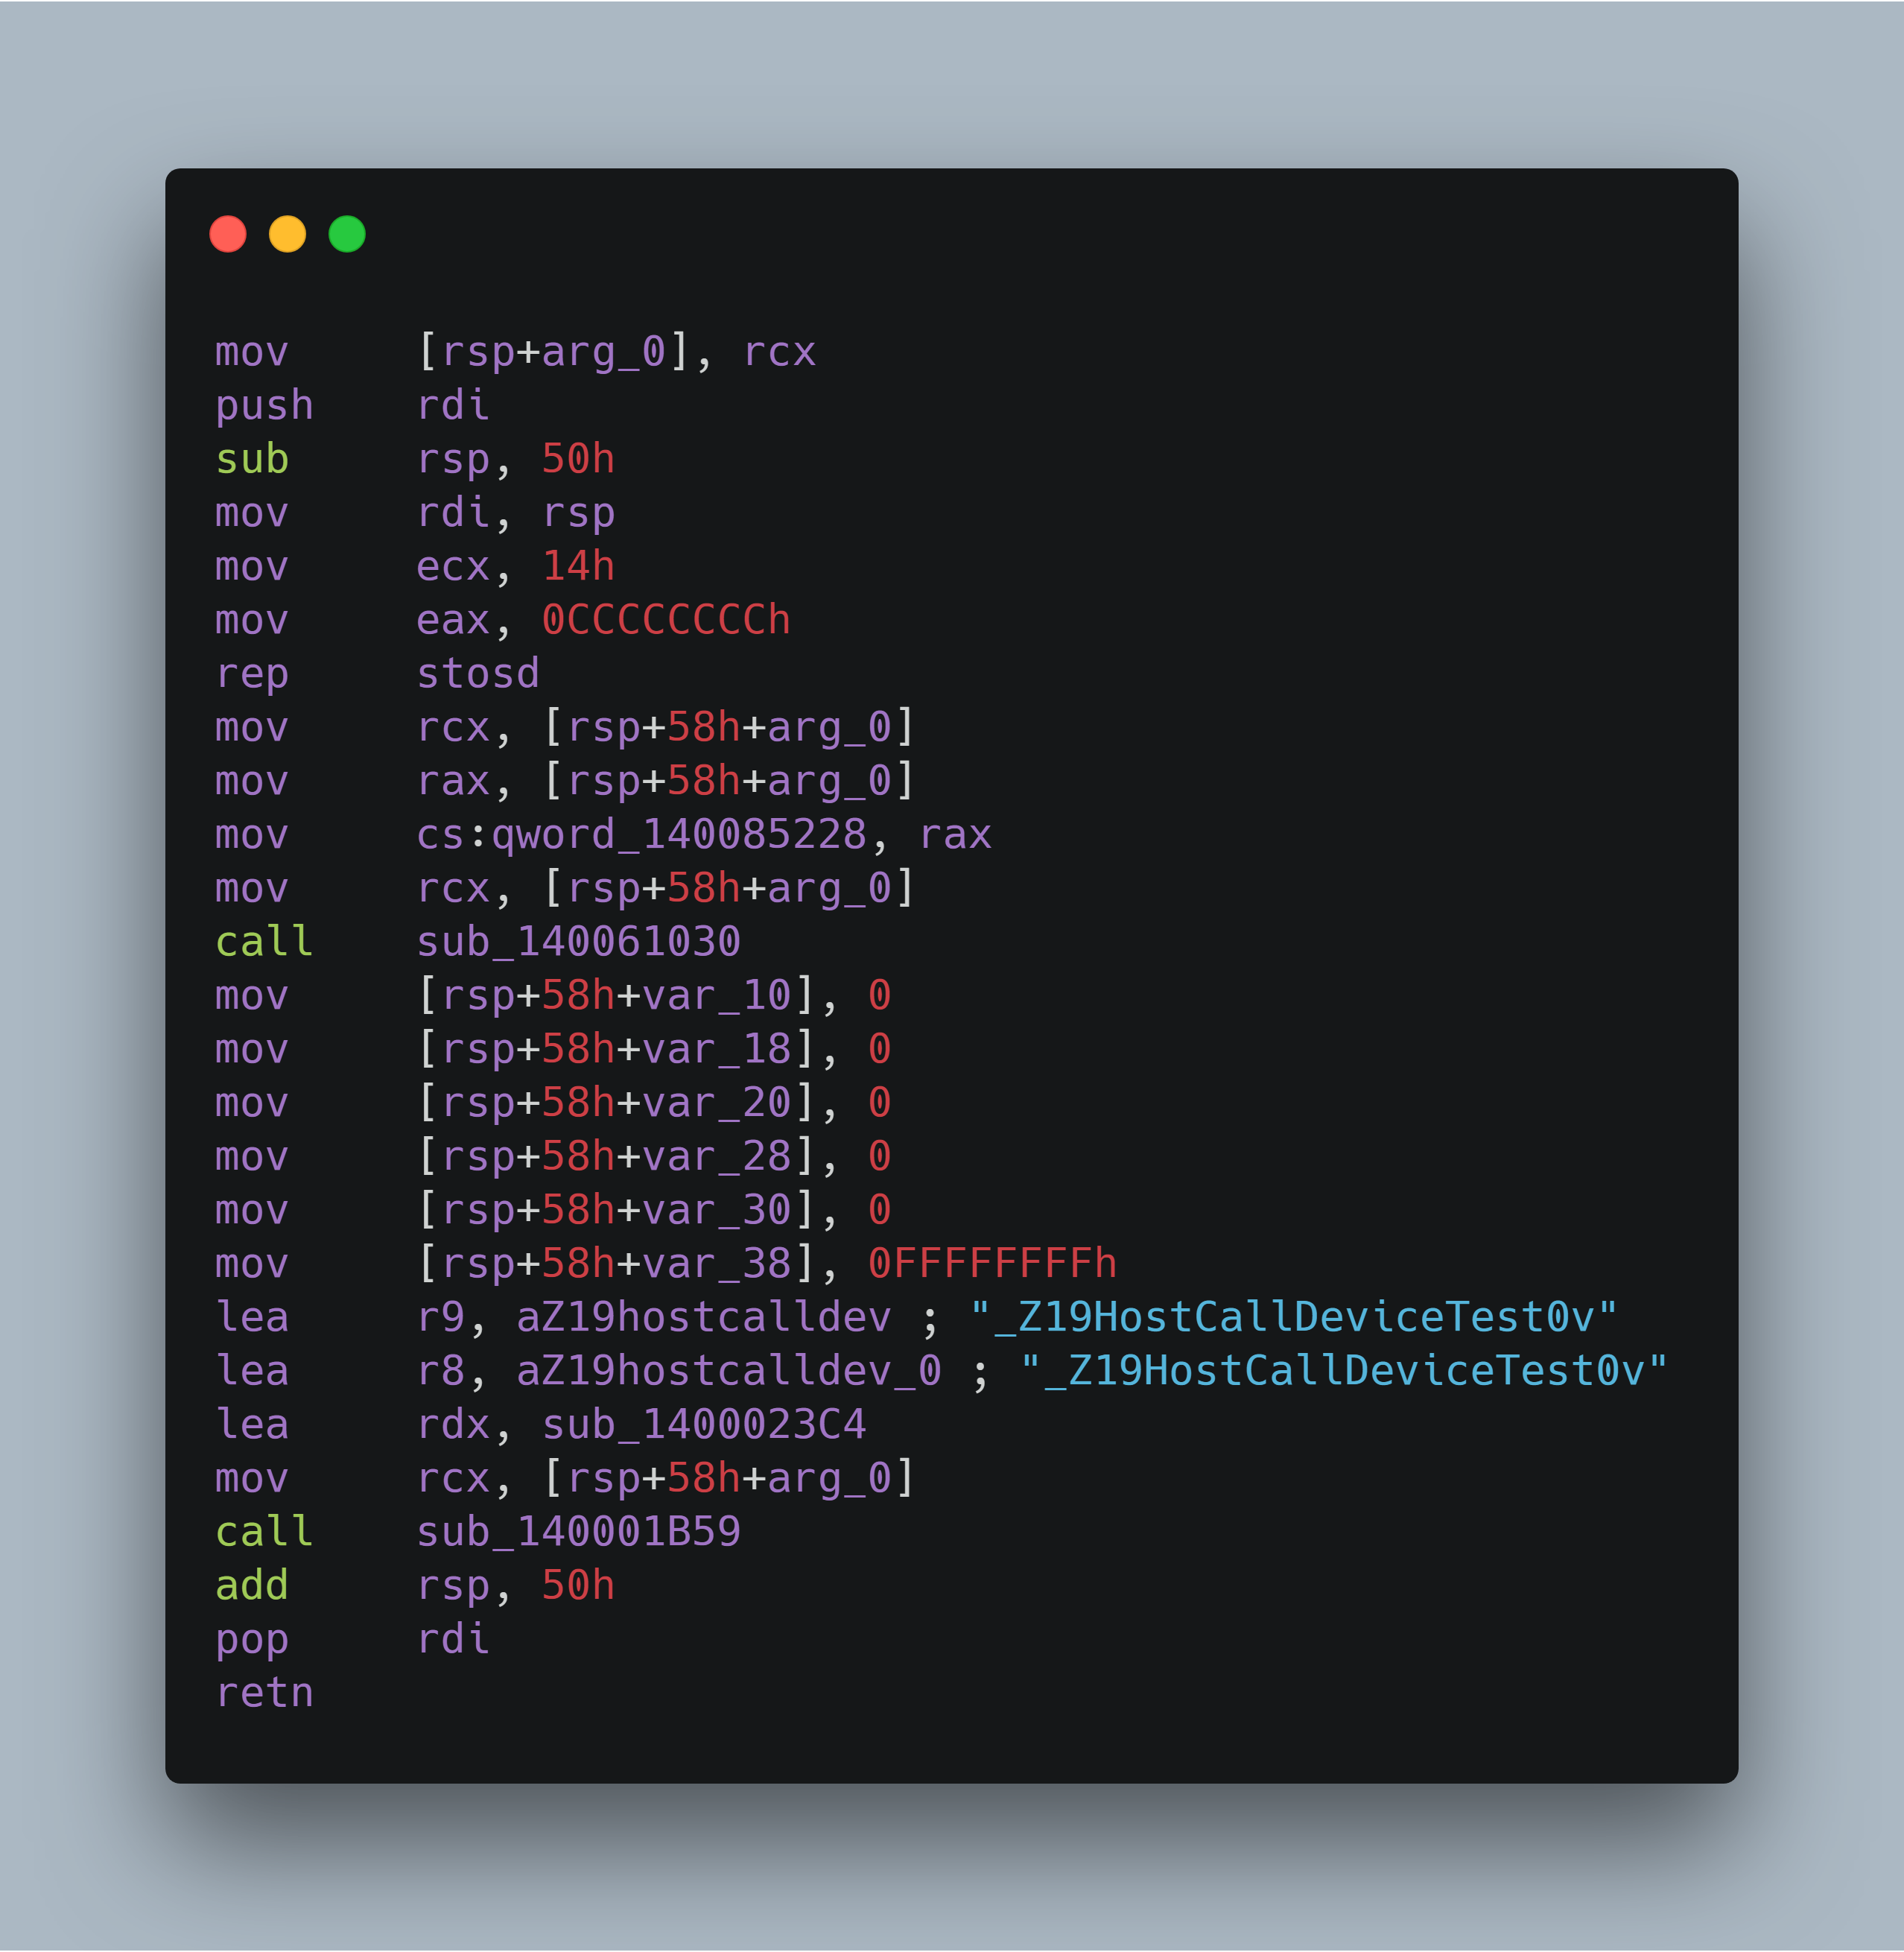
\includegraphics[width=15cm]{figures/CODE4.png}
	\renewcommand{\thefigure}{\arabic{section}-\arabic{figure} }
	\renewcommand{\figurename}{图}
	\caption{CUDA程序部分反汇编代码}
	\addtocounter{figure}{-1}
	\renewcommand{\thefigure}{\arabic{section}-\arabic{figure} }
	\renewcommand{\figurename}{Figure}
	\caption{Part of assembly code of CUDA application}
	\label{Fig.CUDA-Assembly}
\end{figure}
\par 这一节通过CUDA程序在x86\_64架构的CPU下使用静态反汇编生成的汇编代码说明涉及运行于GPU的核函数的调用与返回方式、控制权转交方式等。
\begin{itemize}
\item CUDA中三种函数只有被\_\_global\_\_修饰的函数在讨论范围内,因为只有这种函数跨越CPU与GPU,该函数被称为内核函数(Kernel Function)。调用核函数的加载过程与核函数的地址被存储在数据区(仅有核函数地址,因核函数实际运行于GPU)。
\item 主函数需要定位到核函数加载过程,将核函数加载过程的地址通过lea指令加载进相关寄存器(rcx或rdx),该过程并非被call指令直接调用。
\item 进入加载过程,在执行一系列堆栈检查后,使用call指令调用传递CUDA函数执行时$ <<< >>> $中参数的过程。
\item 正式将核函数地址使用lea指令加载进相关寄存器(r8、r9),然后使用call指令调用正式调用过程,该过程中还包含一系列安全性检查,核函数执行控制权交予GPU,如图\ref{Fig.CUDA-Assembly}所示。
\item 因调用核函数时并非用call指令直接调用,而是使用lea指令加载地址进入寄存器,故CPU端不会等待核函数返回,而是直接执行之后的函数或语句。
\item \_\_device\_\_修饰的函数调用都在PTX代码中。
\end{itemize}

\subsubsection{PTX中间代码结构}
\par PTX(Parallel Thread eXecution)代码是一种底层的并行线程执行虚拟机代码,但这种代码可以直接运行在目标硬件;实际在运行时,PTX代码会编译成更为底层的SASS代码,由于涉及企业机密,此处不再详述。关于CUDA程序的调用、执行方式,线程调度等内容已经在2.1.2节中详细描述,这里只介绍编译生成的PTX代码的简单语法和文件结构。
\par PTX代码有两种语句:Directive Statement和Instruction Statement,前者起到申明的作用,以.开头,如.entry, .func, .extern, .reg等,后者则是具体ALU动作,如add, div, idp4等。在这些语句后需要指明进行操作的值的类型以及位数,如.reg	.f32就是申明了32位float的寄存器变量,.global	.b32就是申明了32位整数的全局内存变量。因Directive Statement在PTX代码中起到寻找函数入口、观察优化方法(比如将全局内存使用优化为寄存器使用)起到非常重要的作用,所以下表详细列出了一些Directive Statement以及相应作用。而ALU动作则较为直观,且大部分为算术运算,这里就不在赘述\parencite{PTX}。
\begin{table}
	\centering
	\renewcommand{\thetable}{\arabic{section}-\arabic{table} }
	\renewcommand{\tablename}{表}
	\caption{部分PTX代码关键词及含义}
	\addtocounter{table}{-1}
	\renewcommand{\thetable}{\arabic{section}-\arabic{table} }
	\renewcommand{\tablename}{Table}
	\caption{Part of PTX keywords and meanings}
	\begin{tabular}{cc}
		\toprule
		项目	&	内容	 \\
		\midrule
		.target & 指明目标硬件的架构和平台 \\
		.address\_size & 指明PTX代码所能访问的地址空间 \\
		.entry & 指明作为入口的核函数地址以及函数体 \\
		.func & 函数定义(包含被CPU调用和GPU的函数) \\
		.branchtargets & 指明潜在的分支目标(线程束分化用) \\
		.calltargets & 表明潜在的被调用目标 \\
		.extern & 可见的外部符号的申明(如C中的extern) \\
		.weak & 可见的外部符号申明(weak指优先级低于global等) \\
		.pragma & 将控制权转交给后台PTX编译器 \\
		.max[nreg,…] & 最大可用的寄存器文件大小,等 \\
		
		\bottomrule
	\end{tabular} \label{table-PTX关键词}\\
	
\end{table}
\par PTX代码的结构较为简单,开头有若干Directive Statement用于指定目标平台和硬件架构等:
\begin{lstlisting}[language={[ANSI]C},numbers=left,numberstyle=\tiny,%frame=shadowbox,  
rulesepcolor=\color{red!20!green!20!blue!20},  
keywordstyle=\color{blue!70!black},  
commentstyle=\color{blue!90!},  
basicstyle=\ttfamily] 
.version 6.3			// 指明PTX代码的版本
.target sm_35, debug		// 指明编译模式和目标硬件架构
.address_size 64		// 指明最大可用地址空间
\end{lstlisting}
之后就是一些列函数入口,包含相当于main函数的:
\begin{lstlisting}[language={[ANSI]C},numbers=left,numberstyle=\tiny,%frame=shadowbox,  
rulesepcolor=\color{red!20!green!20!blue!20},  
keywordstyle=\color{blue!70!black},  
commentstyle=\color{blue!90!},  
basicstyle=\ttfamily] 
.visible .entry _Z19HostCallDeviceTest0v()
.extern .func (.param .b32 func_retval0) vprintf()
.visible .func (.param .b32 func_retval0) _Z21DeviceCallDevice-Test0i()

\end{lstlisting}
\par 该程序片段中,第一行的函数时CPU调用GPU的入口。其函数签名与根据exe文件反汇编出的汇编代码中的函数签名应一致,如图\ref{Fig.CUDA-Assembly}所示。第二行为外部符号,在CUDA中无需实现;第三行则为由设备调用、运行于设备的函数,故没有.entry关键字。
\par 注意在生成函数时会出现\_Z19、\_Z21等字样和i、v等后缀,这是由编译器产生函数签名的方法所致,不同编译器产生的函数签名不尽相同,本文使用的编译器为Microsoft VS。在本文进行的研究中,主要重点放在作为PTX入口的由CPU调用的GPU函数(由\_\_global\_\_修饰)以及由GPU调用的GPU函数(由\_\_device\_\_修饰),而外部符号除涉及GPU全局内存、共享内存、寄存器文件等申请、访问、释放的API等,别的外部符号不做过多讨论。
